% !TEX root = main.tex

The results of the analysis can be sumarised in Figure \ref{fig:waterfall}...


\begin{figure}[H]
\begin{center}
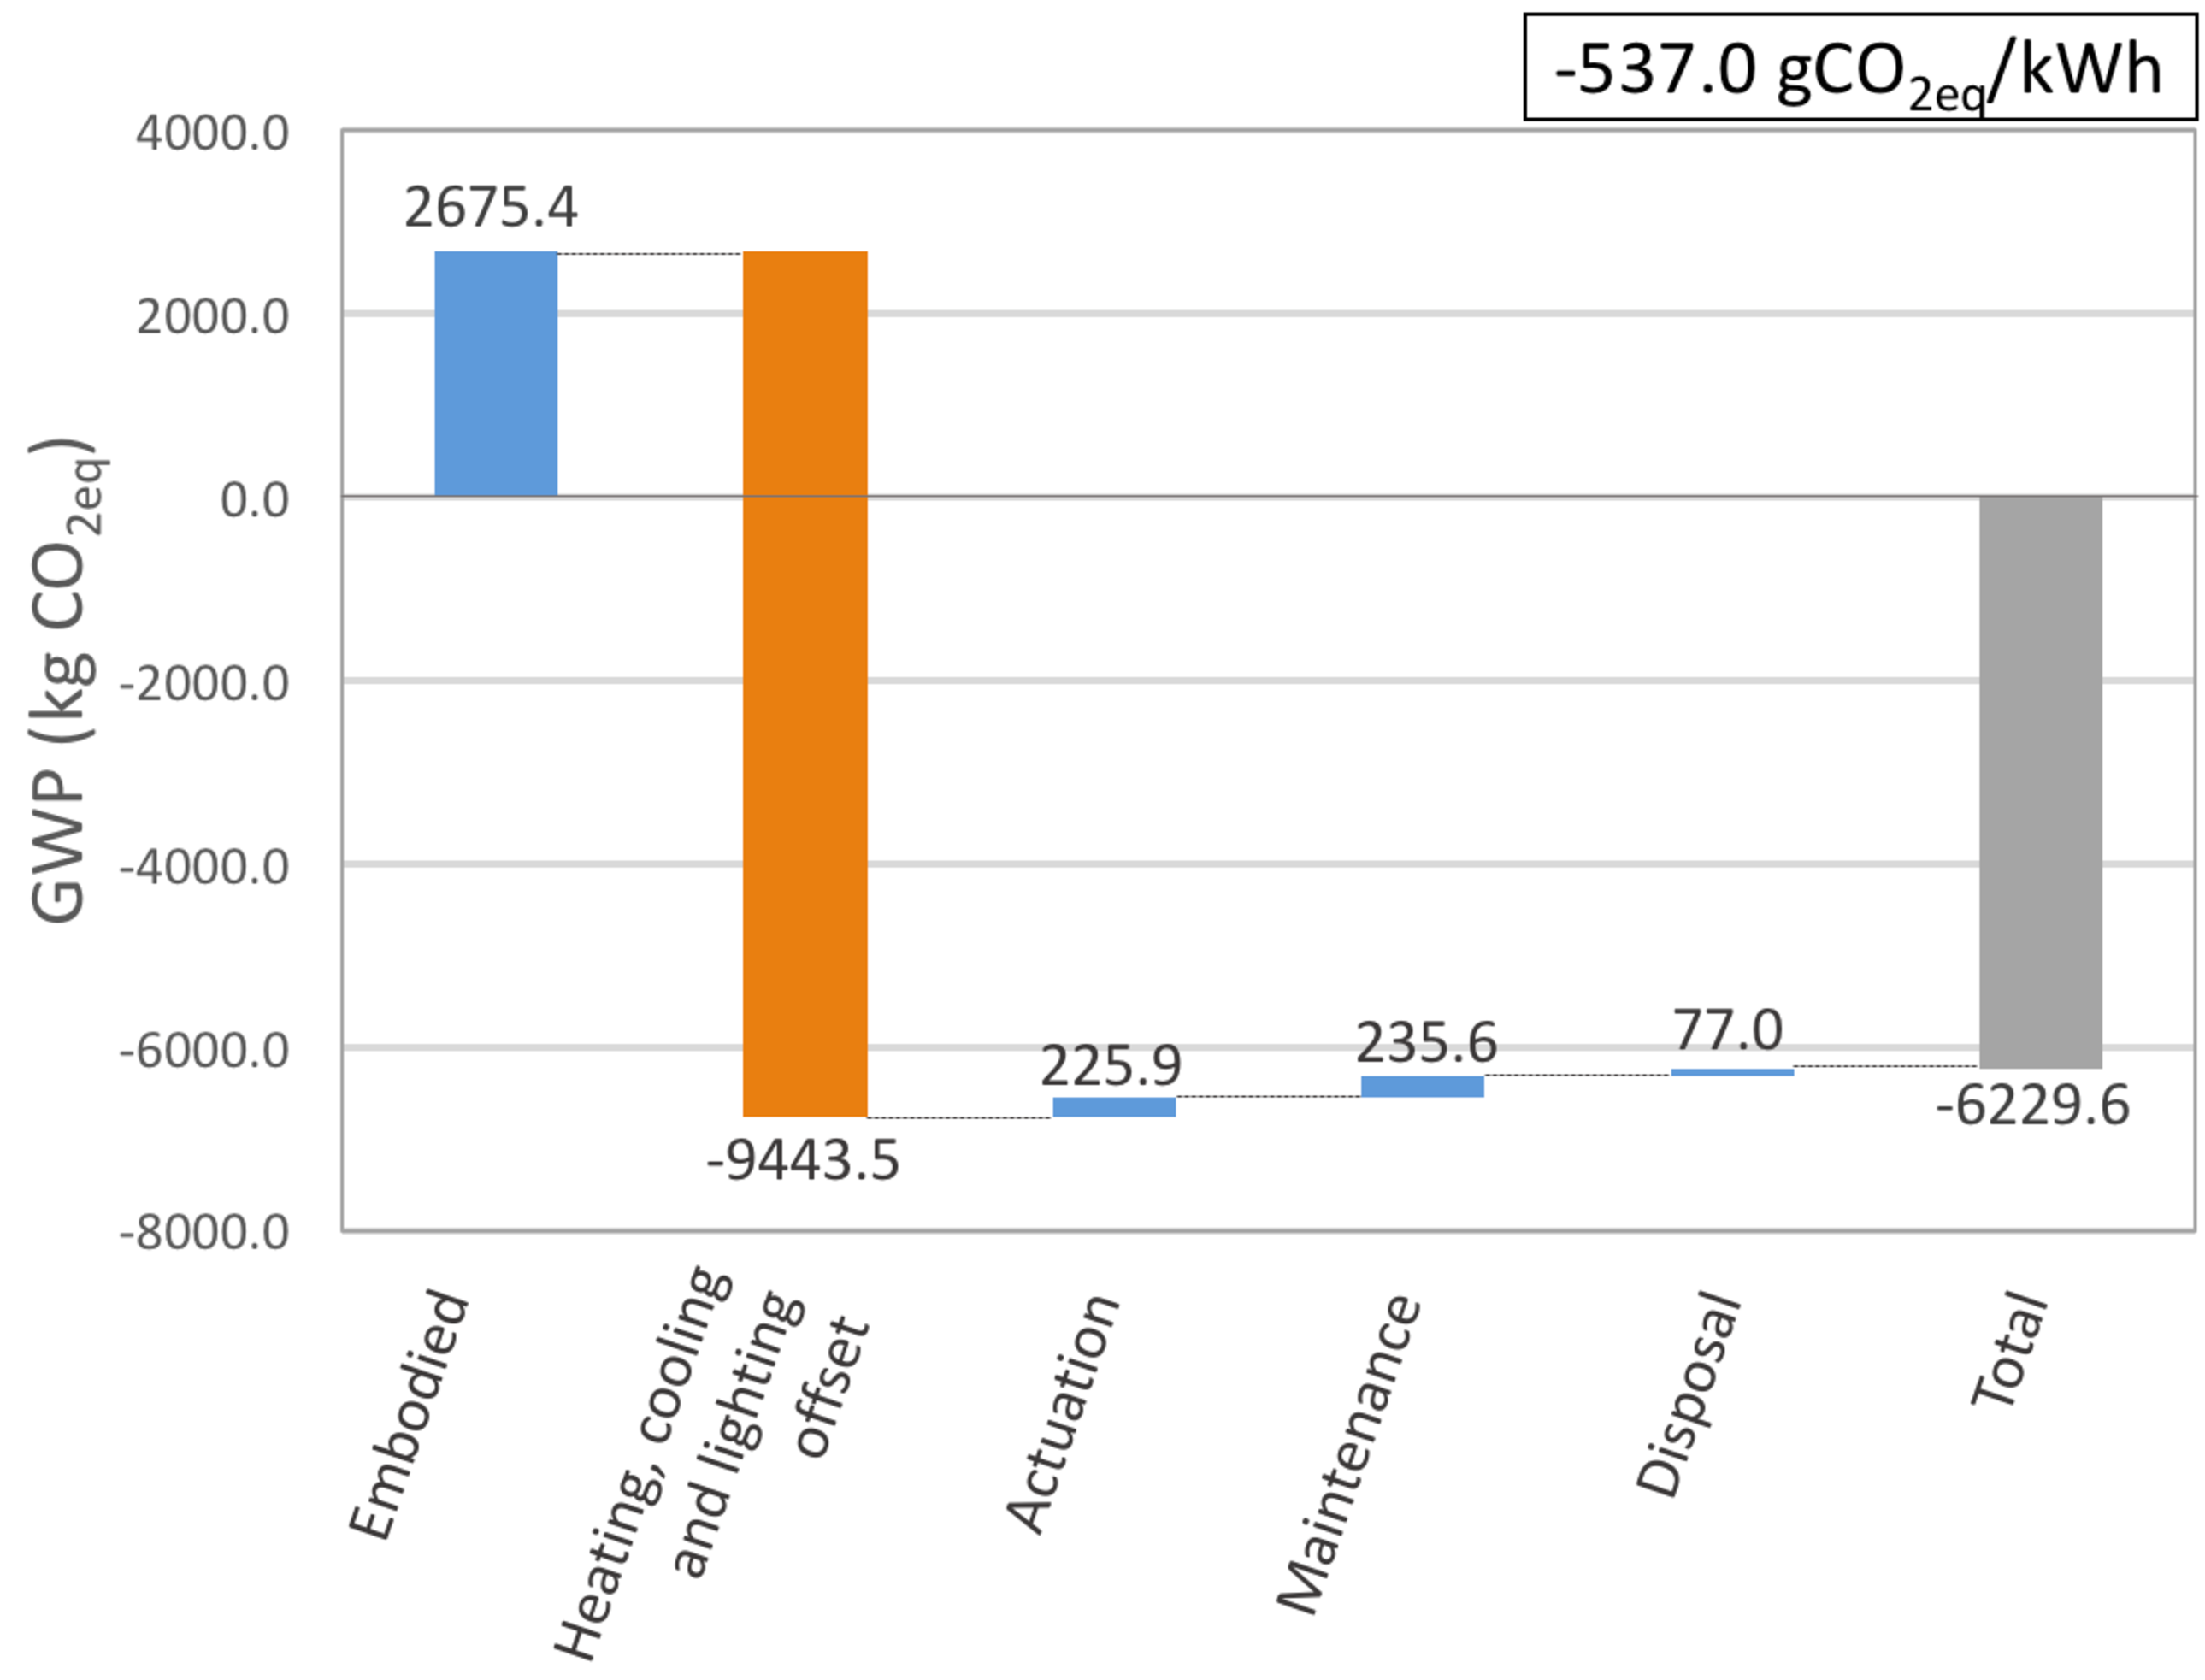
\includegraphics[width=10cm, trim= 0cm 0cm 0cm 0cm,clip]{waterfall}
\caption{Build-up of total GWP of the ASF}
\label{fig:waterfall}
\end{center}
\end{figure}

\begin{figure}[H]
\begin{center}

\includegraphics[width=10cm, trim= 0cm 0cm 0cm 0cm,clip]{monte}
\caption{Monte carlo simulation based on input uncertainties}
\label{fig:monte}
\end{center}
\end{figure}

\begin{figure}[H]
\begin{center}

\includegraphics[width=10cm, trim= 0cm 0cm 0cm 0cm,clip]{sensitivity}
\caption{Sensitivity analysis based on sourcing location}
\label{fig:sensitivity}
\end{center}
\end{figure}
